%%%%%%%%%%%%%%%%%%%%%%%
% User Study Material %
%%%%%%%%%%%%%%%%%%%%%%%

\chapter{Material zur Nutzerstudie}

\section{Aufgabenstellung}
\label{sec:user-study-material-task-description}

\foreach \i in {1,...,5}{

\fbox{\includegraphics[page=\i, width=\textwidth]{resources/user-study-exercises}}

}

\section{Fragebogen}
\label{sec:user-study-material-questionnaire}

\foreach \i in {1,...,4}{

\fbox{\includegraphics[page=\i, width=\textwidth]{resources/user-study-questionnaire}}

}

\section{Auswertung}
\label{sec:user-study-material-evaluation}

\fbox{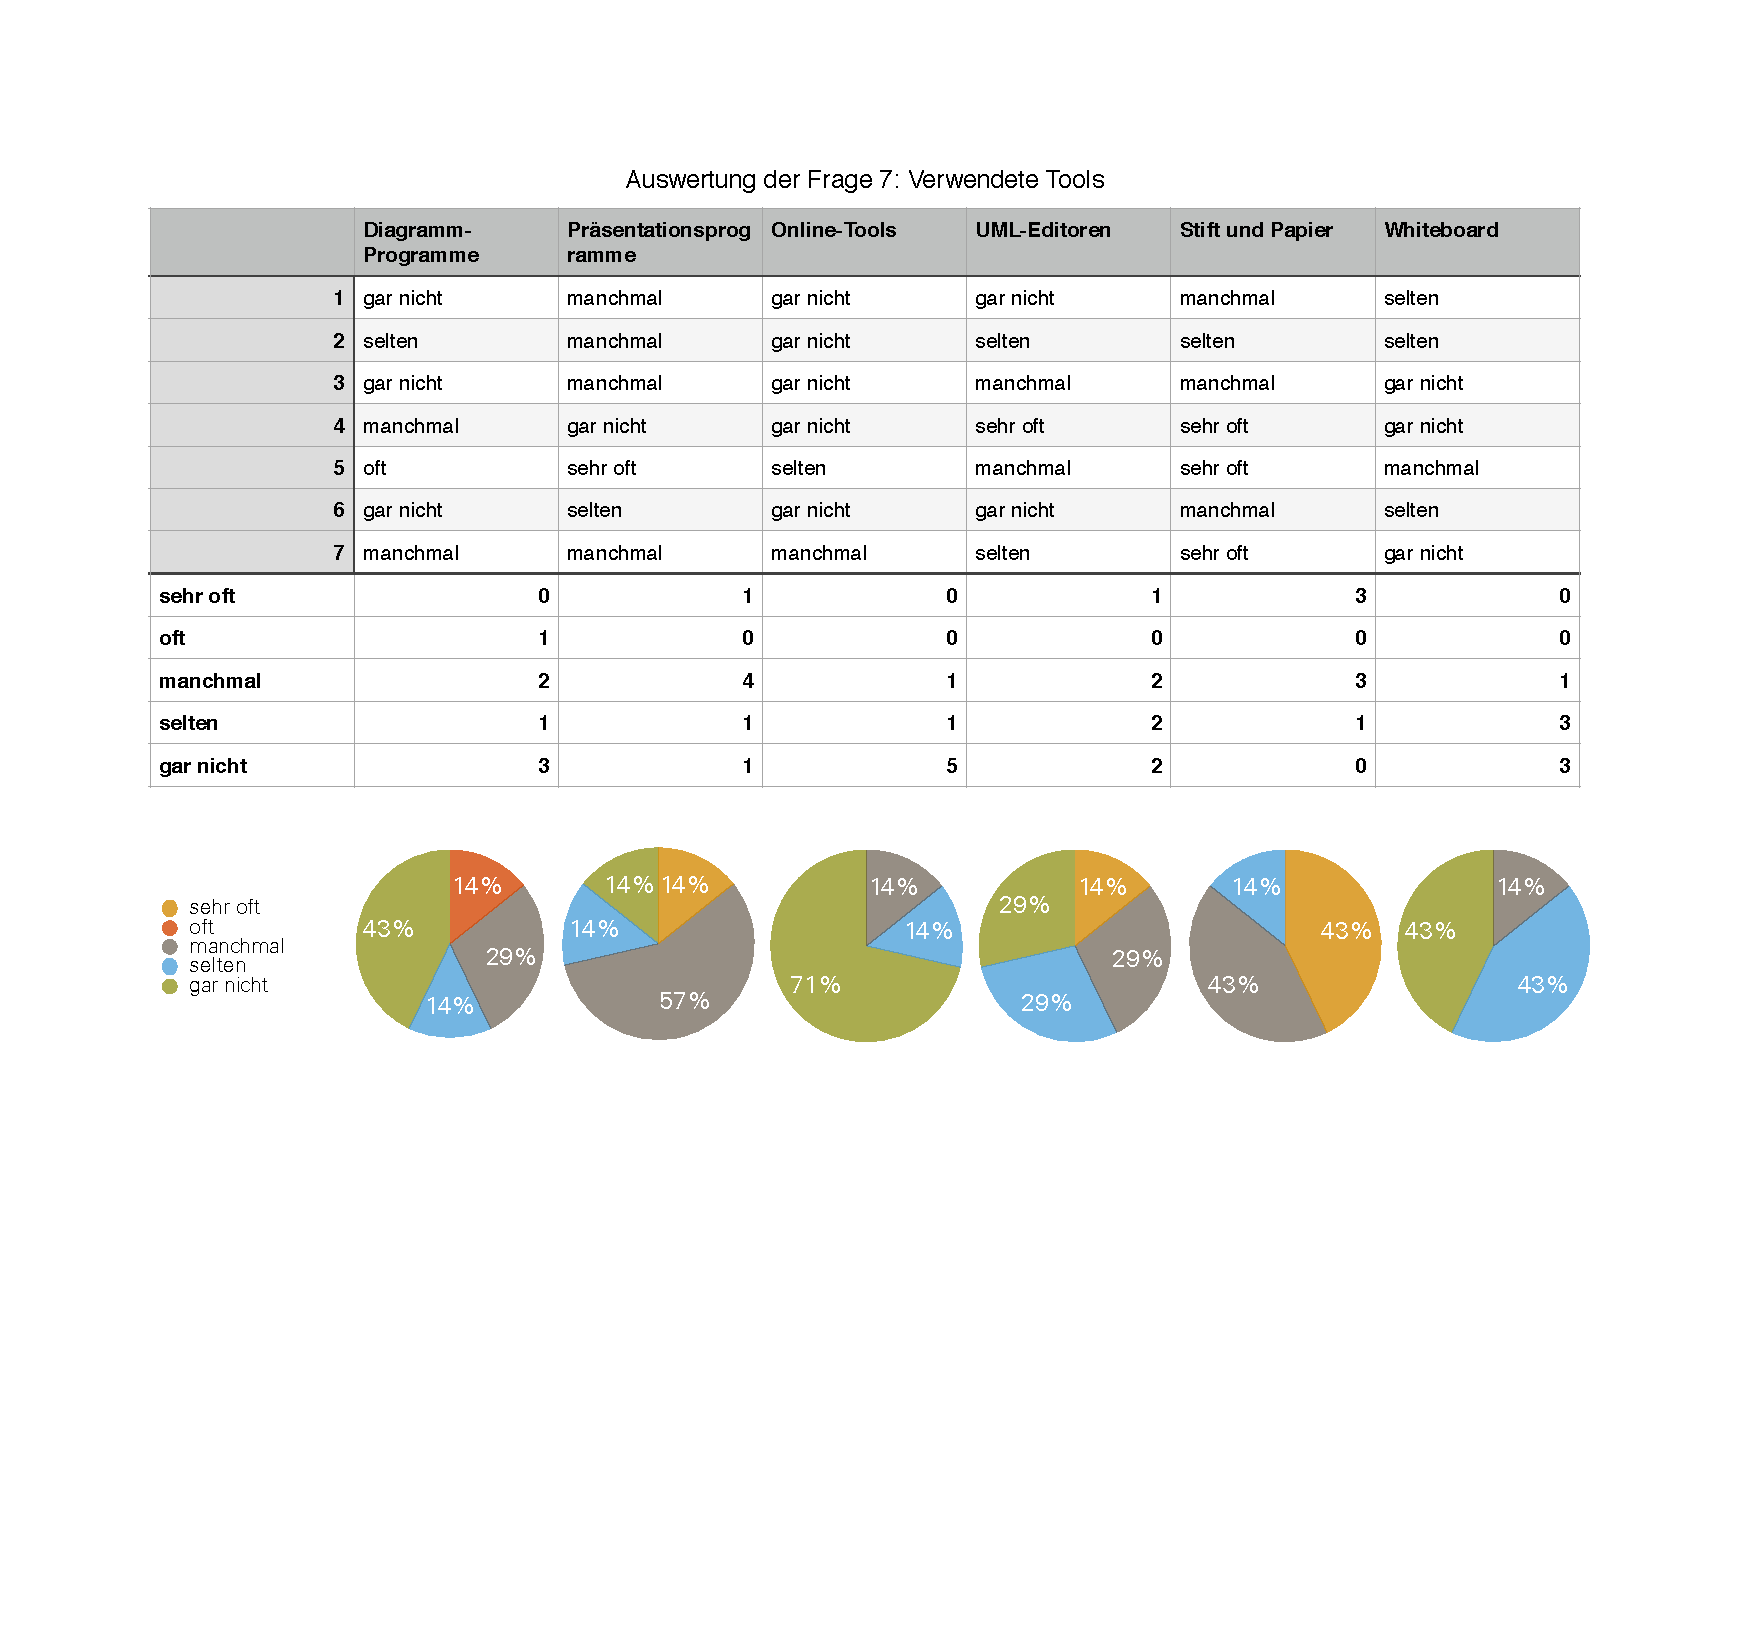
\includegraphics[page=1, width=\textwidth, trim={2cm 9.5cm 2cm 2cm}, clip]{resources/user-study-evaluation}}

\fbox{\includegraphics[page=3, width=\textwidth, trim={1.8cm 8cm 2cm 2cm}, clip]{resources/user-study-evaluation}}

\begin{center}
\fbox{\includegraphics[page=2, scale=0.535, trim={1.8cm 5.5cm 2cm 2cm}, clip, angle=90]{resources/user-study-evaluation}}
\end{center}
